% This file is part of the stream_information project.
% Copyright 2017 the authors. All rights reserved.

% # style notes
% - it is Cram\'er--Rao not Cram\'er-Rao. And yet Fisher-matrix not Fisher--matrix.

% TODO:
% - Reference for the dustmaps package? See software section.

% Story:
% - progenitor - show std_v, std_phi2
% - 2 gaps, 1 under-density - epicycles/streakline? percentiles in polynomial
% - spur - encounter?

\documentclass[modern]{aastex62}

\usepackage{amsmath}

% typography
\setlength{\parindent}{1.\baselineskip}
\newcommand{\acronym}[1]{{\small{#1}}}
\newcommand{\package}[1]{\textsl{#1}}
\newcommand{\gaia}{\textsl{Gaia}}
\newcommand{\pans}{\textsl{Pan-STARRS}}
\newcommand{\DR}{\acronym{DR2}}
\newcommand{\msun}{\rm M_\odot}
\newcommand{\article}{\textsl{Letter}}

% aastex parameters
% \received{not yet; THIS IS A DRAFT}
%\revised{not yet}
%\accepted{not yet}
% % Adds "Submitted to " the arguement.
% \submitjournal{ApJ}
\shorttitle{GD-1 in Gaia DR2}
\shortauthors{price-whelan \& bonaca}

%@arxiver{}

\begin{document}\sloppy\sloppypar\raggedbottom\frenchspacing % trust me

\title{A first look at the GD-1 stellar stream with Gaia DR2}

\author[0000-0003-0872-7098]{Adrian~M.~Price-Whelan}
\affiliation{Department of Astrophysical Sciences,
             Princeton University, Princeton, NJ 08544, USA}
\email{adrn@astro.princeton.edu}
\correspondingauthor{Adrian M. Price-Whelan}

\author[0000-0002-7846-9787]{Ana Bonaca}
\affil{Harvard--Smithsonian Center for Astrophysics, Cambridge, MA 02138, USA}


\begin{abstract}\noindent % trust me
Tidally-disrupted globular clusters are transformed into thin, dynamically-cold streams
of stars that are extremely valuable tracers of the large- and small-scale
properties of mass around the Galaxy.
Most of such streams discovered in the Milky Way reside in its halo, and are therefore primarily sensitive to the distribution of dark matter.
% Many thin stellar streams have been discovered around the Milky Way, the
% majority of which exist in the Galactic halo and are therefore primarily
- cleanest sample, foreground removed w gaia parallaxes; members selected on combination of gaia pm and panstarrs colors
- we thus got the crispest view of the stream to date, revealing in high resolution the rich structure which was only hinted at in the previous generation of data
% We present astrometric data for one of the longest stellar streams --- the
% GD-1 stream --- from the second data release (\DR) of the \gaia\ mission.
% We re-discover significant density variations along the stream by selecting
% candidate member stars using the exquisite \gaia\ data alone, including the
% existence of a prominent, apparent gap in the stream.
% <Using photometric data from the \pans, we refine our selection ...>
These density variations --- and especially the gap --- are possible indications
of past interactions with large, massive perturbers.
<estimate the mass of interaction...>
%
% Many thin stellar streams have been discovered around the Milky Way, the
% majority of which exist in the Galactic halo and are therefore primarily
% sensitive to the distribution of dark matter.
% Here we present astrometric data for one of the longest stellar streams --- the
% ``GD-1'' stream --- from data release 2 (\DR) of the \gaia\ mission.
% We re-discover significant density variations along the stream by selecting
% candidate member stars first using only the exquisite \gaia\ data.
% Combined with filtering using Pan-STARRS photometry, we see clear evidence of
% multiple prominent under-densities and haps in the stream.
% These density variations --- and especially the gaps --- are possible
% indications of past interactions with large, massive perturbers.
% Given that the orbit of the stream crosses the Milky Way disk at large radius,
% these perturbers are likely halo objects and would have to have masses XX,
% suggestive of dark matter sub-halos.
\end{abstract}

\keywords{Galaxy: halo --- dark matter}

\section{Introduction}
\label{sec:intro}

Dynamically cold stellar streams are formed from the tidal disruption of stellar
systems by the gravitational field of their host galaxy (e.g.,
\citealt{Johnston:1998}).
The phase-space density and mean track of stars in streams therefore encode
information about the underlying distribution and shape of mass on galactic
scales (\citealt{Bonaca:2018}).
Most stellar streams are found in the halos of galaxies and are therefore
important tracers of the large-scale distribution of dark matter in galactic
halos.

Streams formed from globular cluster systems are particularly useful as they can
theoretically remain coherent for tens of orbital periods, depending in detail
on the symmetries of the underlying galactic mass distribution
(\citealt{Erkal:...}).
This makes them excellent laboratories for studying small-scale structures in
the mass distribution, as it is expected that density perturbations caused by
interactions with massive perturbers can persist and remain visible for close to
their survival time (e.g., \citealt{Yoon:2011}).
In this sense, streams represent one of the most promising directions for
studying or ruling out the existence of small-scale dark matter sub-halos, as
would be predicted by standard $\Lambda$ Cold Dark Matter ($\Lambda$CDM) theory
(\citealt{Erkal, Sanders, Bovy} papers).

While globular cluster streams are hard to detect around distant galaxies
because of their low relative surface density, over 30 candidate stellar streams
have been discovered throughout the halo of the Milky Way, largely thanks to
large-area, multi-band photometric surveys (e.g., the Sloan Digital Sky Survey,
SDSS; \citealt{York:2000, TODO}).
The Milky Way streams have a wide range of properties such as length, velocity
dispersion, and density (e.g., \citealt{SoManyPeople,Bonaca:2012}; see also the
recent review \citealt{Grillmair:2016, Newberg:2016}), and the majority have no
obvious, bound progenitor systems; Of the thin, likely globular-cluster-origin
streams, only two have clear progenitors (NGC 5466 and Palomar 5; \citealt{TODO,
TODO}).

The most prominent and longest (in angle) thin stream is the GD-1 stream, named
after its discoverers (\citealt{Grillmair:2006}).
GD-1 was found by matched-filtering photometry from the SDSS and spans over
$60^\circ$ in Heliocentric sky coordinates, partially because of its relative
closeness to the sun ($\approx 7$--$10~\textrm{kpc}$).
Despite its proximity, no remnant progenitor cluster or stellar system has been
found associated with the stream.
[Long, somewhat close: useful for constraining large-scale potential (\citealt{Koposov:2009})]

[Small velocity dispersion (quote number?), likely old, retrograde orbit far
from galactic disk, so prime place to search for relics of past subhalo
interactions]
[Known density wiggles and blah (\citealt{DeBoer:2017}), but color-magnitude only, bin stars]

In this \article, we present the cleanest view of the GD-1 stream using
astrometric data from the \gaia\ mission data release 2 (\DR).
Combined with photometry from \pans\ ...
We revisit...do not try to model or fit for Galactic potential. Focus on stream properties, data.

\section{Data}
\label{sec:data}

- Transform to GD-1 coordinates (Koposov et al.)
    - Can see deviation from great circle
- Cut to be close to latitude = 0
- Cut to get proper motion over-density
- Color-magnitude filtering

Figure 1:
- PM cut (panel a)
- PM + CMD cut (panel b)
- SFD (panel c)??

Comment on these here - add figure for both in Appendix?
- Dust / no significant extinction - combine with other figure
- Scanning pattern - just discuss, no figure

Most of the clearly identifiable portions of the GD-1 stream are located at high
Galactic latitudes ($b > 35^\circ$), and we therefore do not expect significant
dust extinction or variations in extinction along the stream.
\figurename~\ref{fig:sfd} shows the $V$-band extinction in the region around the
GD-1 stream, computed from the Schlegel-Finkbeiner-Davis extinction map
(\cite{Schlegel:1998}; hereafter SFD).
Vertical lines indicate the two regions clearly identifiable as under-densities
from the proper-motion-selected stream members.
The maximum $A_V$ is $\approx$0.07 mag in both the under-density and gap
regions.
The dispersion in $A_V$ in the region $-60^\circ < \phi_1 < 0^\circ$ and
$-1^\circ < \phi_1 < 1^\circ$ is $\sigma_{A_V} \approx 0.03~\textrm{mag}$.

% Notebook: GD1-dust-and-completeness
\begin{figure}[h]
\begin{center}
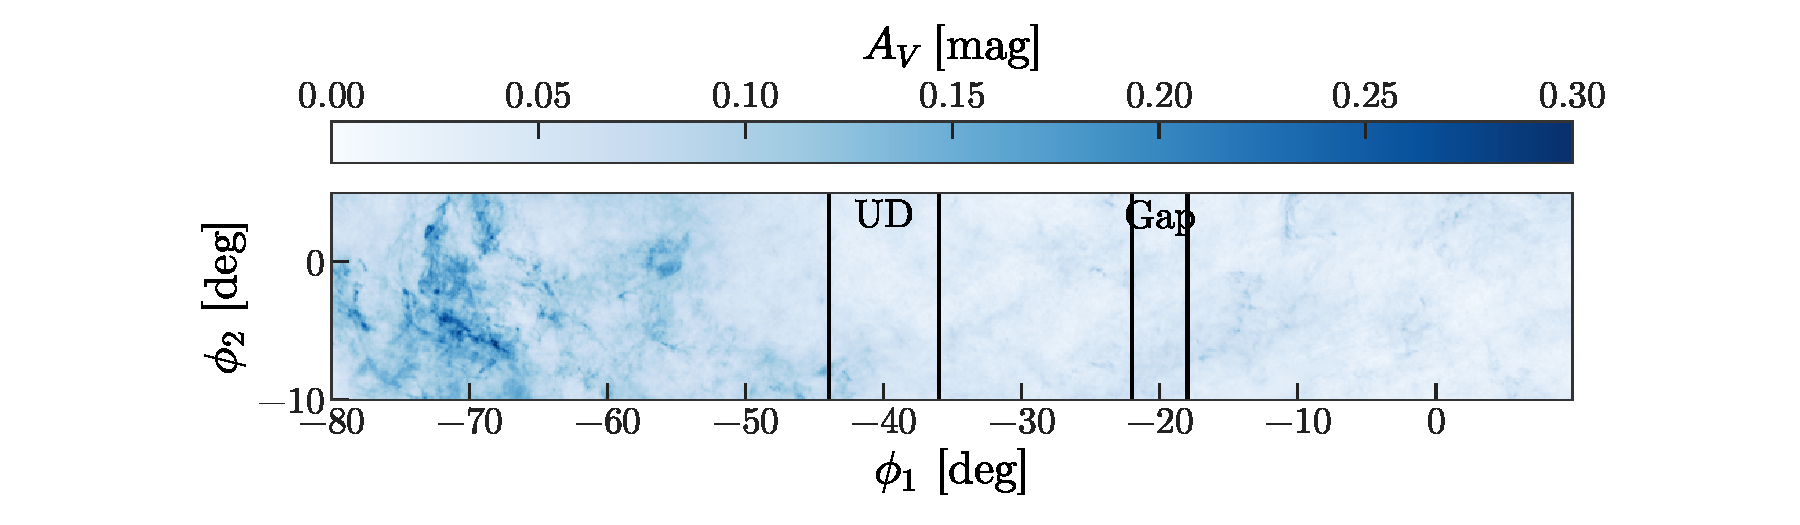
\includegraphics[width=\textwidth]{sfd.pdf}
\end{center}
\caption{%
Colored background shows the $V$-band extinction, $A_V$, in the GD-1
coordinate system.
Vertical lines roughly show the extents the identified under-density (UD) and
gap.
The maximum extinction in the UD or Gap regions is $\approx$0.07 mag.
\label{fig:sfd}
}
\end{figure}


\section{Results}
\label{sec:results}

\subsection{Global properties}
\label{sec:res_global}

\subsection{Gap}
\label{sec:res_gap}

\subsection{Underdensity}
\label{sec:res_underdensity}


\section{Discussion}
\label{sec:discussion}


\acknowledgements{
Gaia
Belokurov, Casey, Geha, Hogg, Johnston, Koposov, Lisanti, Schlafly, Spergel
This research was started at the NYC Gaia DR2 Workshop at the Center for Computational Astrophysics of the Flatiron Institute in 2018 April.
AB acknowledges generous support from the Institute for Theory and Computation at Harvard University.
All code used in this work and all results are available at \url{https://github.com/adrn/GD1-DR2}.
}

\software{
    \package{Astropy} \citep{astropy},
    \package{dustmaps}\footnote{\url{https://github.com/gregreen/dustmaps}},
    \package{gala} \citep{gala},
    \package{IPython} \citep{ipython},
    \package{matplotlib} \citep{mpl},
    \package{numpy} \citep{numpy},
    \package{scipy} \citep{scipy}
}

\bibliographystyle{aasjournal}
\bibliography{gd1}

\clearpage

\appendix
\section{Completeness check and data validation}
\label{sec:validate}

% % Notebook:
% \begin{figure}[h]
% \begin{center}
% \includegraphics[width=0.7\textwidth]{nvisits.pdf}
% \end{center}
% \caption{%
% TODO
% \label{fig:TODO}
% }
% \end{figure}


\end{document}
